\graphicspath{{images/}}

This section present an evaluation of \mad on a real case, the
commissioning of OpenStack. As in the previous section, all results
presented below can be reproduced by following a publicly available
lab\footnote{\url{https://gitlab.inria.fr/VeRDi-project/madeus-journal/lab}}. First,
this lab offers the possibility to reproduce the figures presented in
this section from the raw data obtained in our experiments on
Grid'5000. Second, the lab outlines the complete process to reproduce
the experiments on the Grid'5000 platform.

%------------------------------------
\subsection{OpenStack}
\label{subsec:openstack}
%------------------------------------

OpenStack is the de facto standard open-source solution to address the
IaaS level of the cloud paradigm, in other words OpenStack can be seen
as the open-source operating system of the cloud. Since $2010$, its
community has gathered nearly $700$ organizations (such as Google, IBM
or Intel) and has produced more than $20$ million lines of code. Its
adoption is still growing in various domains such as public
administration, e-commerce and
science\footnote{See \url{http://superuser.openstack.org/} for further
information.}.

OpenStack is a large distributed software system that brings together
almost $100$ software projects. Various projects are in charge of
specific aspects of the infrastructure management (\eg provisioning
virtual machines, providing them with storage, interconnecting them
through networks), and their cooperation is the key to providing the
features required for cloud management.
%
Those projects are themselves composed of several software modules
that are responsible for very specific tasks (\eg placement,
hypervisors, etc.). Although not all are mandatory to deploy an
operable IaaS, $250$ software modules are available in those projects.
%
An OpenStack instance is a composition of some of those modules by the
operator. The chosen modules then cooperate to respond to the operator
requirements. For instance, the operator may need services to manage
virtual rather than bare-metal machines, object storage rather than
file systems, while VLAN networks and billing services may not be
desired in her use case. As defined in the large OpenStack
documentation, each software module has its own commissioning process,
and may depend on other modules commissionings.
%
Thus, the deployment of a typical OpenStack instance involves many
software modules whose commissioning process is characterized by a
large amount of tasks and interplay. As a consequence, the
commissioning process of OpenStack is complex to understand and can be
very long when tasks are executed sequentially.

\kolla is one of the most popular tools for deploying OpenStack in
production.  It relies on \ansible to deploy the modules of OpenStack as
\docker containers, and will be our reference in the
rest of this section.
% SR: not sure what is meant
%It is highly opinionated out-of-the-box,
It allows operators to quickly deploy a basic OpenStack instance, but
also offers complete customization for advanced
administrators. The use case described in this
section corresponds to the default \kolla deployment, which provides
the essential mechanisms to operate an infrastructure with OpenStack.

In the following, we show how the commissioning process of an
OpenStack project can be translated into a \mad component. Leveraging
\mad enables us to express tasks and components coordination. As a
consequence, the \mad modeling improves the clarity of the global
commissioning process, and can be used to reduce commissioning time by
exploiting \emph{SIMH}, \emph{inter-comp}, \emph{inter-comp-tasks}
and \emph{intra-comp-tasks} parallelism levels.

\begin{table*}
  \begin{center}
    
\begin{tabular}{|c|c|c|c|c|}
   \hline
   & Roles & Places & Transitions & Ports \\
   \hline
   Nova & Manages compute instances (\eg Virtual machines) & 5 & 8 & 8\\
   Glance & Compute image store & 3 & 4 & 7\\
   Neutron & In charge of network resources & 3 & 4 & 7\\
   MariaDB & An SQL server used by most projects to store persistent
    information & 4 & 5 & 4\\
   Keystone & Manage user authentication, authorization and service
    discovery & 3 & 2 & 4\\
   RabbitMQ & The message bus for inter-service communication & 2 & 1 & 3\\
   HAProxy & Load-balances the requests to OpenStack controllers & 2 & 1 & 7\\
   OpenVSwitch & Virtualizes network functions & 3 & 1 & 2\\
   MemCached & Caches ephemeral data for most OpenStack projects & 2 & 1 & 2\\
   Facts & Collects informations about every nodes & 2 & 1 & 1\\
   Common & Common utilities (\eg cron, fluentd: a metric collector for logging)
    & 3 & 2 & 2\\
%   \hline
%   Total & 32 & 30 & 47 & \\
%   \hline
%   & Places & Transitions & Ports & Roles\\
%   \hline
%   Nova & 5 & 8 & 8 & Manage compute instances (\eg Virtual machines)\\
%   Glance & 3 & 4 & 7 & Compute image store\\
%   Neutron & 3 & 4 & 7 & In charge of network resources\\
%   Keystone & 3 & 2 & 4 & Manage user authentication, authorization and service
%    discovery\\
%   MariaDB & 4 & 5 & 4 & An SQL server used by most projects to store persistant
%    information\\
%   RabbitMQ & 2 & 1 & 3 & The message bus for inter-service communication\\
%   HAProxy & 2 & 1 & 7 & Load-balances the requests to OpenStack API services\\
%   OpenVSwitch & 3 & 1 & 2 & Virtualizes network functions\\
%   MemCached & 2 & 1 & 2 & Caches ephemeral data for most OpenStack projects\\
%   Facts & 2 & 1 & 1 & Collects inforamtions about every nodes\\
%   Common & 3 & 2 & 2 & Common utilities (\eg cron, fluentd: a
%   metric collector for logging) \\
   \hline
   Total & & 32 & 30 & 47\\
   \hline
\end{tabular}


    \caption{Number of places, transitions and ports for each \mad component
        of the OpenStack assembly of Figure~\ref{fig:full}. 
        \emph{intra-comp-tasks} (\texttt{ICT}) indicates if parallel transitions 
        exist in the component.}
    \label{tab:os}
  \end{center}
\end{table*}

To compare the performance of \kolla and \mad, we have defined $11$
\mad components based on the \ansible roles defined in \kolla's
playbooks (\ie \ansible sequence of components to deploy). Their
names usually indicate the OpenStack project they deploy.
\Cref{tab:os} lists these components and indicates which aspect of the
cloud management they are responsible for.
%

Each of these control components has been designed such that \ansible roles and 
their associated tasks are divided into \mad transitions. \Cref{tab:os} displays 
some metrics for the \mad components designed from \ansible roles of 
\kolla: the number of places, transitions and ports.
%
This table also indicates whether parallel transitions
exist, \ie \emph{intra-comp-tasks} parallelism,
denoted \texttt{ICT}. Additionally, the higher the number of ports, the
more coordination must be performed by \mad during the commissioning. As
depicted in \cref{tab:os}, Nova, Glance, Neutron and MariaDB are
components of particular interest since they contain more transitions
and ports than the others.

%------------------------------------
\subsection{Expressivity and Separation of Concerns}
%------------------------------------

\begin{figure*}
  \begin{center}
    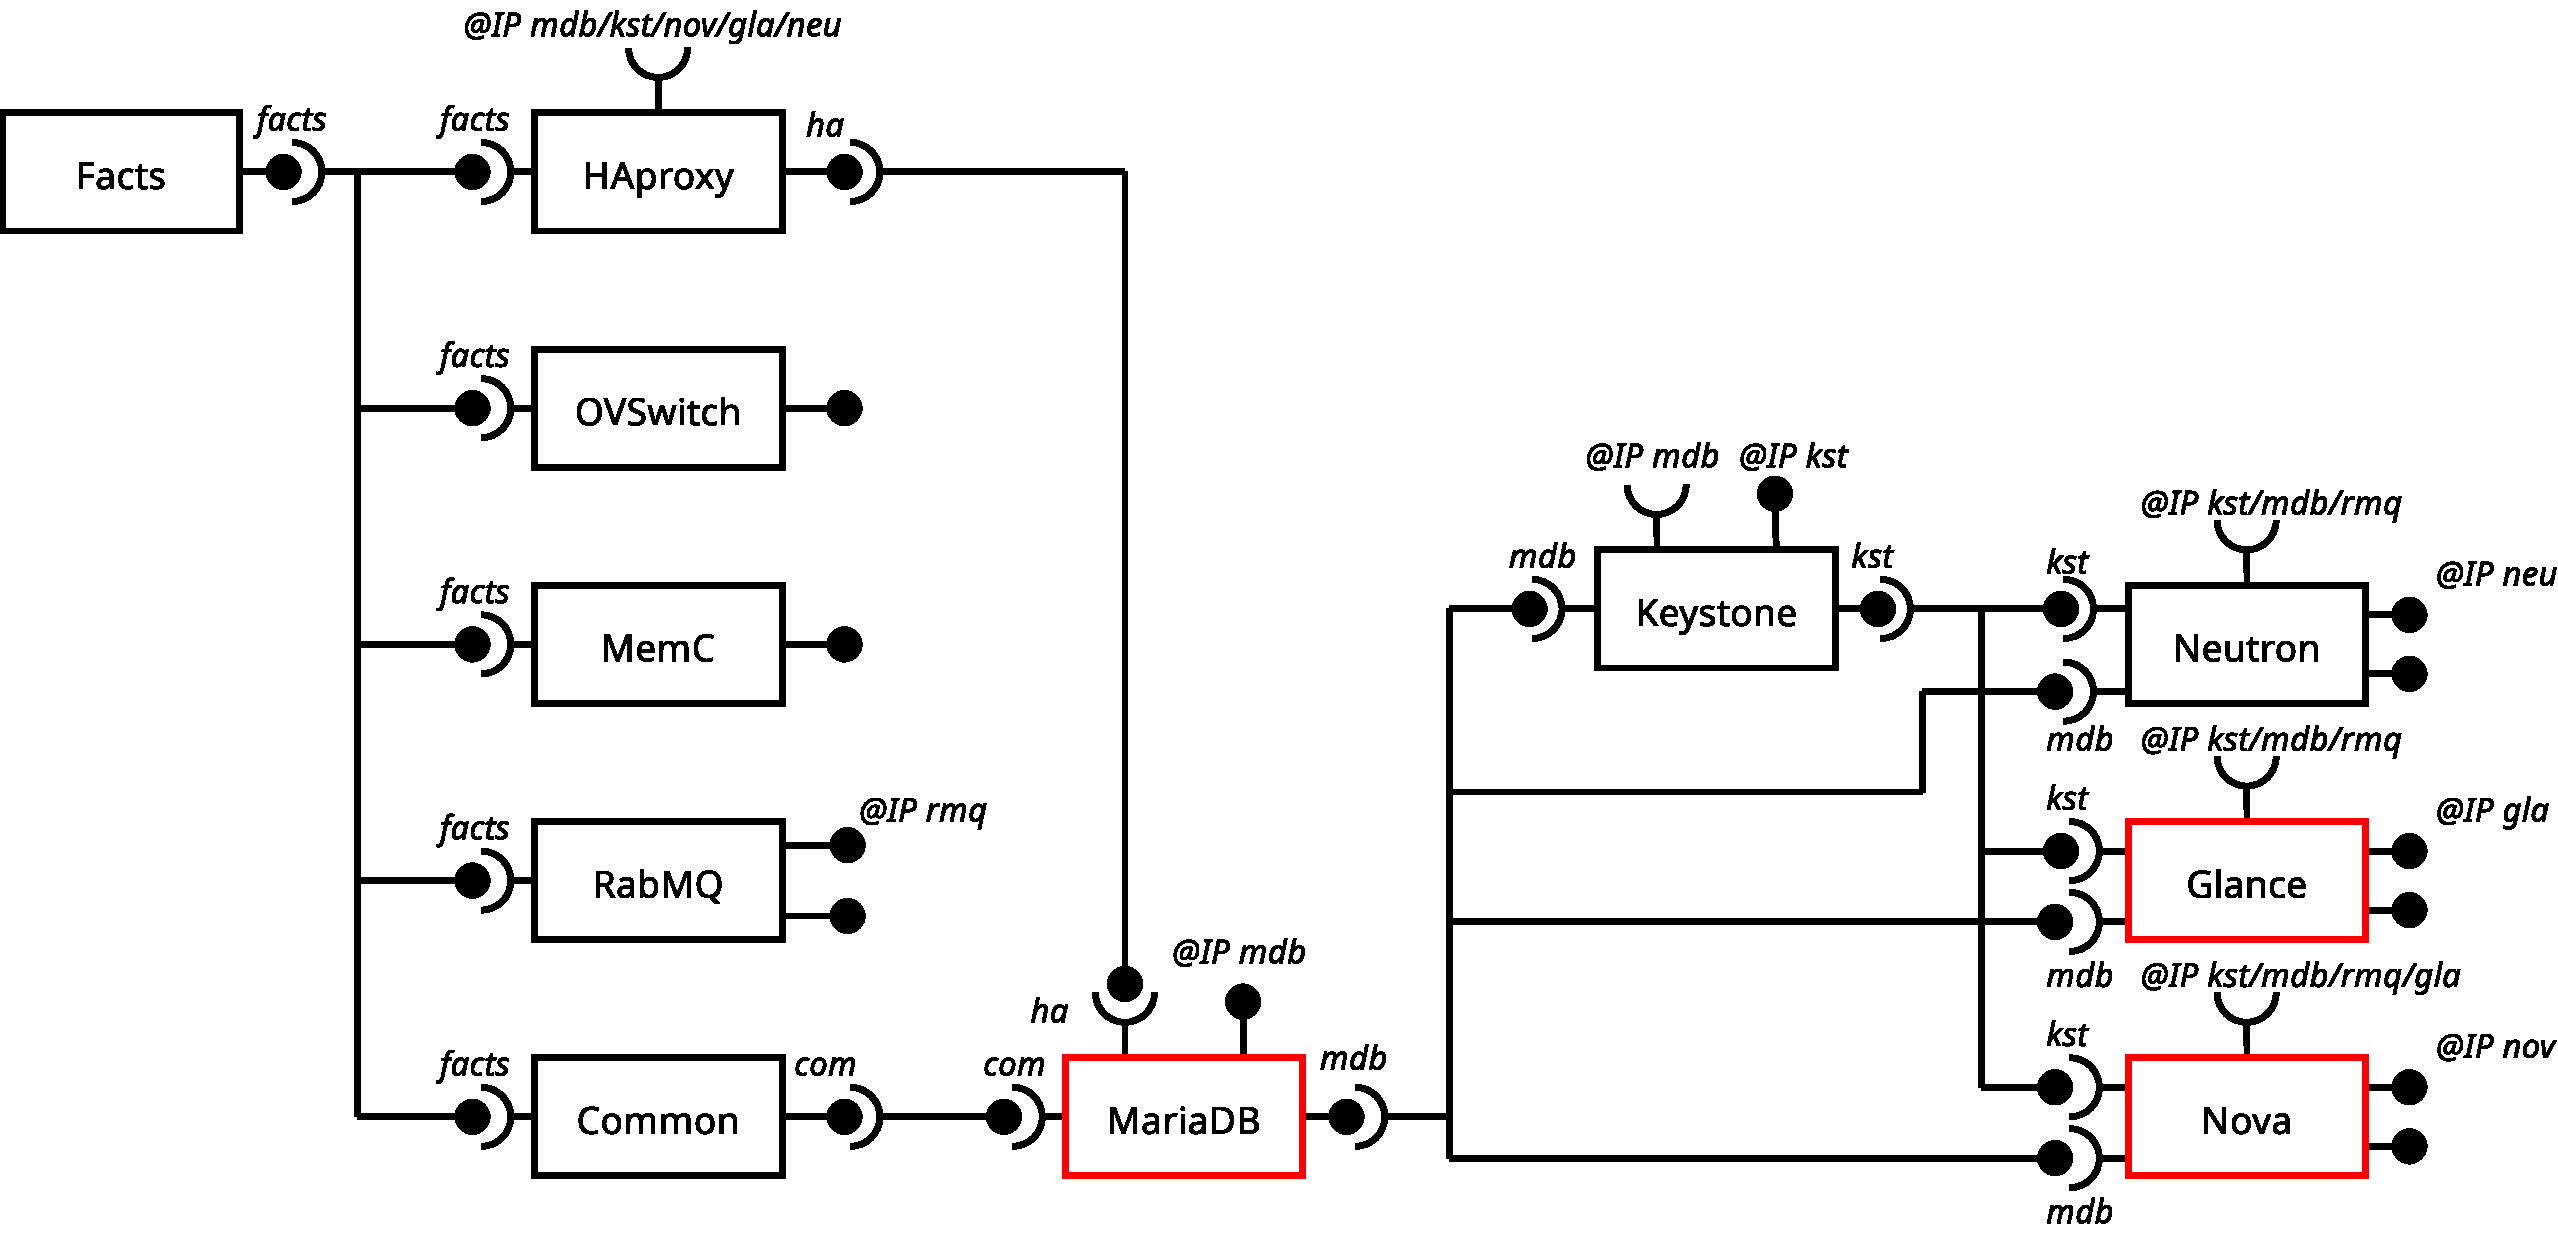
\includegraphics[width=0.7\textwidth]{./images/full2.pdf}
    \caption{Simplified \mad assembly of the \kolla-based OpenStack deployment
    containing $11$ components. Connections between data ports are not depicted.
    Red components are detailed in \cref{fig:sub}.}
    \label{fig:full}
  \end{center}
\end{figure*}

Figure~\ref{fig:full} depicts the use case from the perspective of the sysadmin or devops engineer 
(\ie at the level of the \mad assembly). For the sake of simplicity and 
readability, the connections between ports representing data are not represented. 
This figure helps to understand the high level of interplay between components. 
For instance, Neutron, Glance and Nova require Keystone, while Keystone itself requires 
a database (\ie MariaDB) for its commissioning process. Regarding
separation of concerns, the devops engineer does not need to understand component 
internals. She just needs to compose the desired components by listing them and 
connecting their compatible ports. As a consequence, a component can be replaced 
by another one if they expose the same interfaces. For instance the operator could 
replace MariaDB with MySQL, another component that also implements a database and
exposes the same ports.

\begin{figure*}[t]
  \begin{center}
    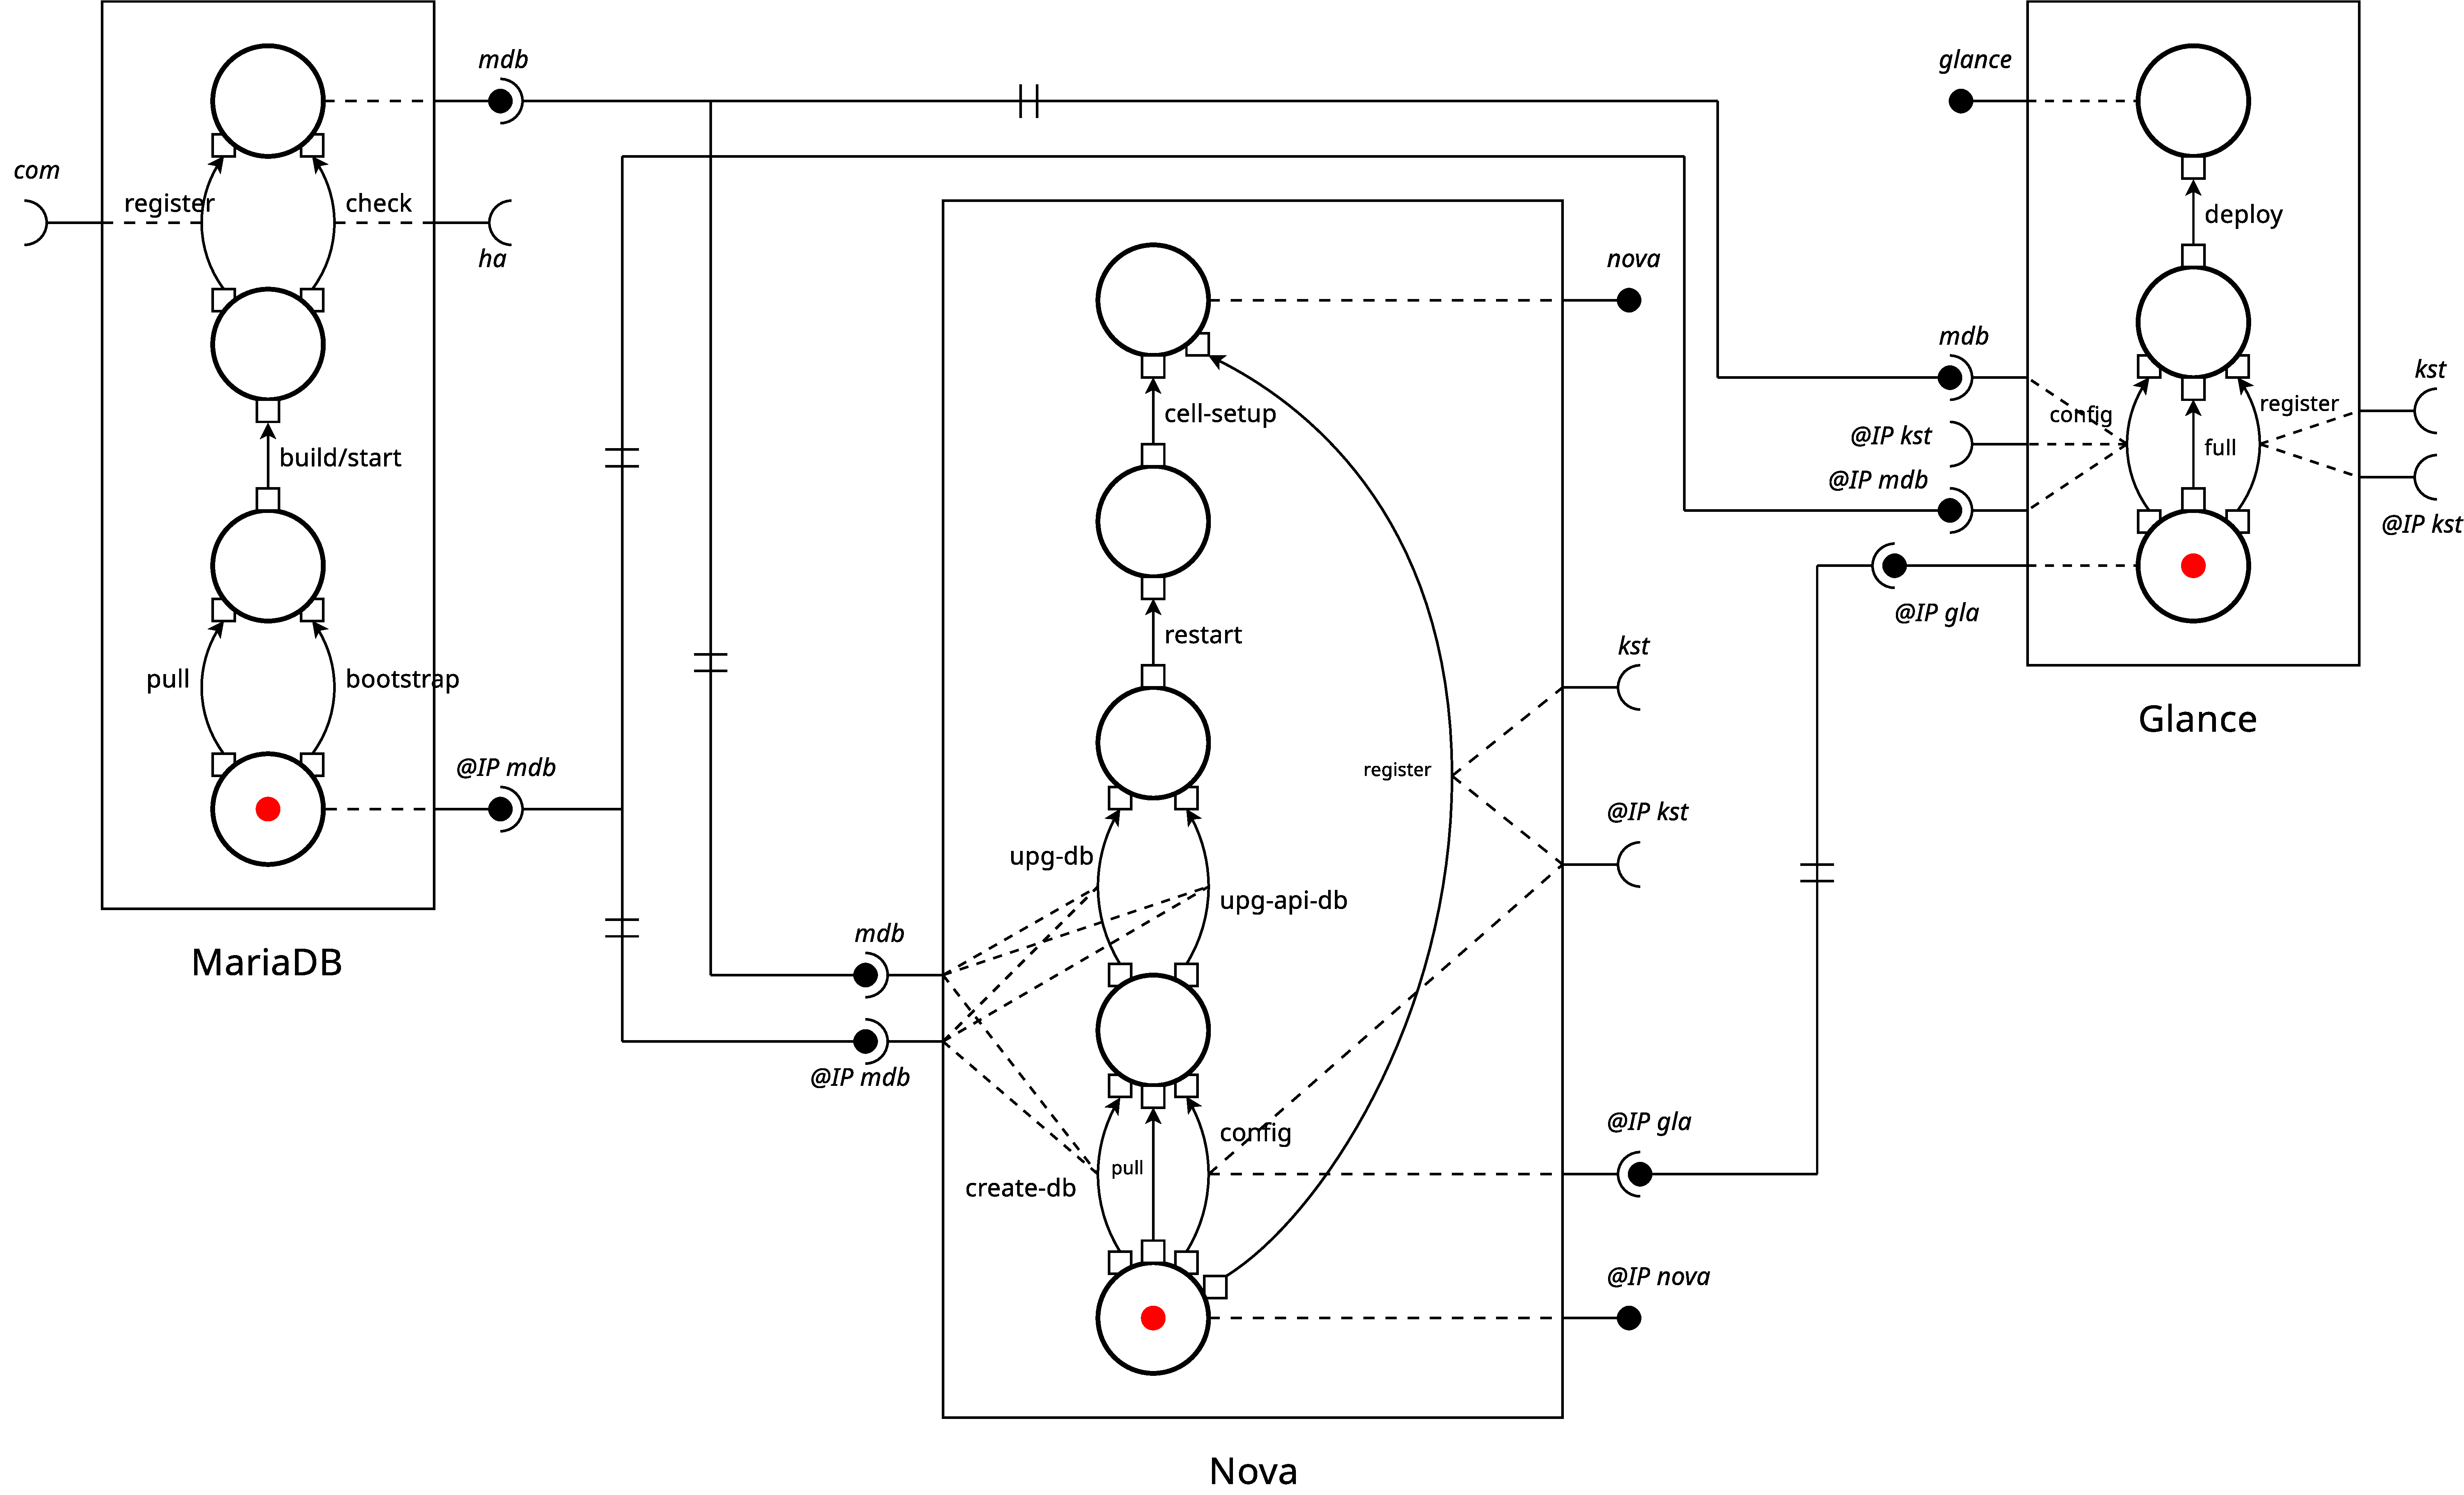
\includegraphics[width=0.8\textwidth]{./images/sub2.pdf}
    \caption{A detailed sub-part of the previous component assembly to deploy
    OpenStack.}
    \label{fig:sub}
  \end{center}
\end{figure*}
%TODO: J'aurais peut être représenté Keystone à la place de MariaDB
%   1. Est-ce utile de dire que mariadb ici est différent de mariadb avant et
%   pas risqué pour embrouiller le message ?
%   2. Register est une transition liée à Keystone qui est très intéressante
%   quand on examine Nova (transition indépendante des autres)

We now study our use case from the perspective of the developer,
focusing on the three colored control components from
Figure~\ref{fig:full}: MariaDB, Nova and Glance. Figure~\ref{fig:sub}
depicts the internals and interactions of these components.

The dependencies previously observed at the assembly level are more
detailed at the developer level. For instance, if we isolate Nova and Glance,
Figure~\ref{fig:full} lets us think that Glance
must be deployed before Nova, but it is clear here that once Nova obtains
Glance's IP address (provided by the first place in Glance), both
components can be deployed in parallel. This shows how \mad can be
leveraged for \emph{inter-comp} and \emph{inter-comp-tasks}
parallelism. In addition, as discussed previously,
Figure~\ref{fig:full} suggests that MariaDB must be deployed before Keystone,
and Keystone before Neutron, Glance and Nova. However, the \mad
representation depicted in Figure~\ref{fig:sub} shows that
only the \emph{register} transition of Glance and Nova requires the
Keystone catalog service to be available (\ie to register themselves
in the catalog). We see on the figure that other tasks can be
executed in parallel, while \emph{register} waits for Keystone (\eg for
Nova, this transition is independent from all others).
Similarly, Figure~\ref{fig:sub} depicts many
parallel transitions for each component, showing how \mad can be leveraged for
\emph{intra-comp-tasks} parallelism in this use case.

%------------------------------------
\subsection{Experimental Setup and Parameters}
% ------------------------------------

This section first defines the experimental setup: (i) how modules are
distributed among nodes (\ie servers or machines) and (ii) the testbed
characteristics. Then we describe the parameters used during
our experimentation: (iii) the assemblies we designed to compare our
contribution with the related work and (iv) the way \docker images are
fetched by nodes.

%-------
\paragraph{Node roles and module distribution}
Each of the $11$ components defined earlier in \kolla is in charge of
an OpenStack project. As mentioned, each OpenStack project
contains multiples software modules. Hence, each component actually
deploys different modules ($36$ in total). A basic multi-node \kolla
deployment targets three nodes. First, the \emph{Control} node, which
hosts control services, APIs and databases, deploying $16$
services. The second one is the \emph{Network} node that hosts network
agents and HAProxy, and contains $11$ services. Finally, the
\emph{Compute} node, in charge of compute services and VM placement,
hosts $9$ services.

\begin{table}
  \begin{center}
    \small
    
\begin{tabular}{|c|c|c|c|}
   \hline
   Cluster & CPU & Memory & Network\\
   \hline
   Nova & 2 x Intel Xeon E5-2620 v4 & 64GB & 10Gbps\\
   (lyon) & 8 cores/CPU &  & \\
   \hline
   Taurus & 2 x Intel Xeon E5-2630 & 32GB & 10Gbps\\
   (lyon) & 6 cores/CPU & & \\
   \hline
   Sol & 2 x AMD Opteron 2218 & 4GB & 1Gbps\\
   (sophia) & 2 cores/CPU & &\\
   \hline
\end{tabular}


    \caption{Grid'5000 clusters configurations.}
    \label{tab:g5k}
  \end{center}
\end{table}

%-------
\paragraph{Testbed and resource provisioning}
Our evaluations were conducted on two clusters of the
experimental platform Grid'5000: \ecotype and \nova. \Cref{tab:g5k}
shows the hardware configuration for both clusters. The cluster
\ecotype has better hardware (CPU, memory, networkinterfaces) than \nova,
as described in the table. To design reproducible benchmarks, we used
EnosLib\footnote{\url{https://gitlab.inria.fr/discovery/enoslib}}, a
library to build experimental frameworks on multiple testbeds (\eg
Grid5000, LibVirt), and
Execo\footnote{\url{http://execo.gforge.inria.fr/doc/latest-stable/index.html}},
another library for prototyping experiments. Since \kolla, our
reference, does not manage resource provisioning, we do not include
this phase in the use case, nor in our benchmark. Although resource
provisioning could be managed by \mad, this step is left to EnosLib
and not counted in execution times.

%-------
\paragraph{Assemblies}
Our performance evaluation compares three assemblies that
are designed to capture the behavior of \ansible, \aeolus and \mad. To
that end, the component internals for each assembly vary with regards
to the number of places, transitions and ports. Importantly, we re-used
the \ansible files provided by
\kolla and split them into component transitions. By using \mad to
coordinate \ansible execution, it is possible for us to provide a way
to fairly compare these solutions. Moreover, by using divided \kolla
roles, the \emph{SIMH} parallelism level is handled by \ansible in the
three assemblies.

The first assembly, called \ansass, matches the \kolla-\ansible
commissioning process. Each component is triggered sequentially, in
the same way and order as \ansible triggers sequentially the roles
defined in \kolla. Since the coordination
between components is simply sequential, the components have two states
connected by a single transition which performs all the commissioning
tasks, such as in \kolla (\ie no \emph{intra-comp-tasks}
parallelism). Each time a component is deployed, it activates the
commissioning process of the next one (\ie neither \emph{inter-comp}
nor \emph{inter-comp-tasks} parallelism). This assembly features the
first level of parallelism, which is managed by \ansible when tasks are
mapped to multiple nodes, \ie \emph{SIMH} parallelism.
%

The second assembly, called \aeoass is equivalent to an \aeolus
commissioning of OpenStack. It provides parallelism at both the
\emph{inter-comp} and \emph{inter-comp-tasks} levels in addition to
\emph{SIMH}, and no \emph{intra-comp-tasks} parallelism. Coordination
is performed through component ports. In this assembly, most components are
built with two sequential transitions. When the assembly is
initiated, the first transition of those components are triggered,
while the second one depends on another
component.
%

The third assembly, called \madass, leverages our contribution to
commission OpenStack. It corresponds to the one we previously
described when presenting the use case. Components are defined on a
case-by-case basis, based on our understanding of the OpenStack
commissioning process. As depicted previously in \cref{tab:os}, most
components include multiple places and transitions. This assembly
makes use of all the parallelism expressiveness of \mad.

\begin{table}
  \begin{center}
    
\begin{tabular}{|c|c|c|c|}
   \hline
   & Compute & Network & Control\\
   \hline
   Number of images & $9$ & $11$ & $16$\\
   \hline
   Total Size (MB) & $2767$ & $2705$ & $4916$\\
   \hline
\end{tabular}


    \caption{Number of \docker images per node and their cumulated size in MB to
      download from the registry.}
    \label{tab:images}
  \end{center}
\end{table}

%-------
\paragraph{Docker container registry}
Finally, since \kolla relies on \docker containers, fetching \docker
images has a significant impact on our results: images have to be
downloaded, before being decompressed. To be as neutral as possible we
have conducted experiments with three different modes for handling
those images: (1) \emph{cached} mode, where images are previously
placed on OpenStack nodes, so fetching \docker images has very low impact on
the results; (2) \emph{local} mode, where images are previously
downloaded on a new dedicated node of the cluster, from which images
can be loaded (\ie a local \docker registry); (3) \emph{remote} mode,
in which images are fetched from an Internet repository (\ie the
DockerHub registry). \Cref{tab:images} gives for each OpenStack node
(\ie Compute, Network and Control) the number of \docker images to
download and their compressed size.  As depicted in this table, more
than $10$GB must be downloaded in our use case.  Furthermore, the
control node has to download almost twice as much data as the other
nodes.

%------------------------------------
\subsection{Results}
%------------------------------------

In this section, we analyze the results of our benchmark through
different aspects: (i) the performance of each assembly; (ii) the
adequation between the theoretical predicted performance and the
measured results and (iii) the influence of registry modes on our
results.

\begin{figure}[t!]
  \begin{center}
    \def\svgwidth{\columnwidth}
    \subfloat[Performance comparison on \ecotype]{
      \input{./images/use_case_ecotype_perf.pdf_tex}
      \label{fig:ecotype}
    }
    \def\svgwidth{\columnwidth}
    \subfloat[Performance comparison on \nova]{
      \input{./images/use_case_nova_perf.pdf_tex}
      \label{fig:nova}
    }
    \caption{Recorded time in seconds for OpenStack commissioning with
      different clusters, assemblies and registry modes. Upper parts
      represent mean values with relative ratios for each result
      compared to the reference \ansass.  Lower parts display means,
      standard deviations and the minimum and maximum values computed
      from the theoretical performance model, depicted as boxes.}
    \label{fig:openstack_results}
  \end{center}
\end{figure}

\begin{table}
    \begin{center}
        
\begin{tabular}{cll|ccc}
\toprule
& & & remote & local & cached \\

\midrule
\multirow{9}{*}{\STAB{\rotatebox[origin=c]{90}{measured}}} & \multirow{3}{*}{\STAB{\rotatebox[origin=c]{90}{mean}}}  & ansible  &
529s &
480s &
332s \\
 & & aeolus &
263s &
258s &
229s \\
 & & madeus &
150s &
151s &
133s \\
\cmidrule{2-6}& \multirow{3}{*}{\STAB{\rotatebox[origin=c]{90}{gain}}}  & ansible  &
0\% &
0\% &
0\% \\
 & & aeolus &
50\% &
46\% &
30\% \\
 & & madeus &
71\% &
68\% &
59\% \\
\cmidrule{2-6}& \multirow{3}{*}{\STAB{\rotatebox[origin=c]{90}{std}}}  & ansible  &
2s &
2s &
1s \\
 & & aeolus &
1s &
6s &
1s \\
 & & madeus &
4s &
5s &
4s \\
\midrule
\multirow{6}{*}{\STAB{\rotatebox[origin=c]{90}{theoretical}}} & \multirow{3}{*}{\STAB{\rotatebox[origin=c]{90}{max}}}  & ansible  &
533s &
483s &
335s \\
 & & aeolus &
266s &
275s &
231s \\
 & & madeus &
155s &
157s &
137s \\
\cmidrule{2-6}& \multirow{3}{*}{\STAB{\rotatebox[origin=c]{90}{min}}}  & ansible  &
525s &
477s &
330s \\
 & & aeolus &
261s &
254s &
227s \\
 & & madeus &
143s &
144s &
124s \\
\bottomrule
\end{tabular}
        \caption{Measured and theoretical results of our benchmark on \ecotype.}
        \label{tab:openstack_results_ecotype}
    \end{center}
\end{table}

\begin{table}
    \begin{center}
        
\begin{tabular}{cll|ccc}
\toprule
& & & remote & local & cached \\

\midrule
\multirow{6}{*}{\STAB{\rotatebox[origin=c]{90}{measured}}} & \multirow{3}{*}{\STAB{\rotatebox[origin=c]{90}{mean(s)}}}  & ansible  &
$770 \pm 3$ &
$754 \pm 4$&
$539 \pm 3$\\
 & & aeolus &
$446 \pm 2$&
$434 \pm 3$&
$398 \pm 2$\\
 & & madeus &
$326 \pm 7$&
$317 \pm 5$&
$295 \pm 1$\\
\cmidrule{2-6}& \multirow{3}{*}{\STAB{\rotatebox[origin=c]{90}{gain}}}  & ansible  &
0\% &
0\% &
0\% \\
 & & aeolus &
42\% &
42\% &
26\% \\
 & & madeus &
57\% &
57\% &
45\% \\
%\cmidrule{2-6}& \multirow{3}{*}{\STAB{\rotatebox[origin=c]{90}{std}}}  & ansible  &
%3s &
%4s &
%3s \\
% & & aeolus &
%2s &
%3s &
%2s \\
% & & madeus &
%7s &
%5s &
%1s \\
\midrule
\multirow{6}{*}{\STAB{\rotatebox[origin=c]{90}{theoretical(s)}}} & \multirow{3}{*}{\STAB{\rotatebox[origin=c]{90}{max}}}  & ansible  &
774 &
761 &
541 \\
 & & aeolus &
449 &
440 &
401 \\
 & & madeus &
335 &
321 &
296 \\
\cmidrule{2-6}& \multirow{3}{*}{\STAB{\rotatebox[origin=c]{90}{min}}}  & ansible  &
766 &
750 &
533 \\
 & & aeolus &
444 &
430 &
395 \\
 & & madeus &
319 &
308 &
292 \\
\bottomrule
\end{tabular}
        \caption{Measured and theoretical results of our benchmark on \nova.}
        \label{tab:openstack_results_nova}
    \end{center}
\end{table}


In these studies, we refer to Figures~\ref{fig:ecotype}
and~\ref{fig:nova} which respectively show our results on \ecotype and
\nova clusters. The upper part displays the recorded times to
commission OpenStack as a function of the three studied assemblies.
For a better understanding of the comparison, the value of
each result is written on top of the bars, while the ratio compared to
\ansass, our reference, is displayed below the bars' edges.
Furthermore, for each assembly on the X-axis, the results for the
three \docker registry settings are displayed with different colors:
blue, red and green respectively for \emph{remote}, \emph{local} and
\emph{cached}. On the lower part of the figures, the means for each
result are depicted as blue, red and green horizontal lines, the
related standard deviations are represented by vertical lines, while
boxes represent the minimum and maximum values computed with the
theoretical performance model of Section~\ref{sec:perf_model}.
%\CP{Vérifier d'où vient ces min max value}
%\HC{expliqué plus tard}
% 
For the sake of readability, the scale of the lower parts are
differents for each assembly. Each result corresponds to the average
computed across $10$ iterations. The corresponding numerical values are
also displayed in \cref{tab:openstack_results_ecotype} and \cref{tab:openstack_results_nova}.
%
%\HC[Dimitri]{pourquoi les resultats sur ecotype seulement dans le
%  tableau? mettre 2 tableaux?}
% Et bien ça en fait un beau paragraphe pour seulement expliquer comment
% fonctionne la figure ^^'...

%\CP{Les tableaux font doublons par rapports aux figures -- il y a juste besoin de 
%presenter la difference par rapport aux }
% \HC{oui mais moi comme relecteur j'aime bien avoir les tableaux en plus des 
%figures pour mieux apprécier les chiffres}

%-------
\paragraph{Impact of assemblies}

We now compare the time measured to commission the three assemblies
previously defined: \ansass, \aeoass and \madass (the lower, the
better in Figure~\ref{fig:openstack_results}).  As expected, the time
required to commission these assemblies reflects the level of
parallelism they implement. Since \ansass is limited to the first
parallelism level, \ie \emph{SIMH}, its commissioning time is longer
than \aeoass. By featuring \emph{inter-comp} and
\emph{inter-comp-tasks} parallelism, the latter outperforms the former
from $26$\% (\nova, \emph{cached}) to $50$\% (\ecotype,
\emph{remote}). Leveraging \emph{intra-comp-tasks} parallelism enables
\madass to outperform \ansass~from $45$\% (\nova, \emph{cached}) to
$71$\% (\ecotype, \emph{remote}), and \aeoass from $16$\% (\nova,
\emph{remote}/\emph{local}) to $30$\% (\ecotype, \emph{cached}).
The OpenStack commissioning on \ecotype goes from
almost 9 minutes with \ansass to less than 3 minutes with \madass.
%

\begin{figure*}[t]
	\begin{center}
		%\vspace{-3em}
		\def\svgwidth{\columnwidth}
		\scriptsize
		\subfloat[\ansass with \emph{cached} registry]{
			\scalebox{0.9}{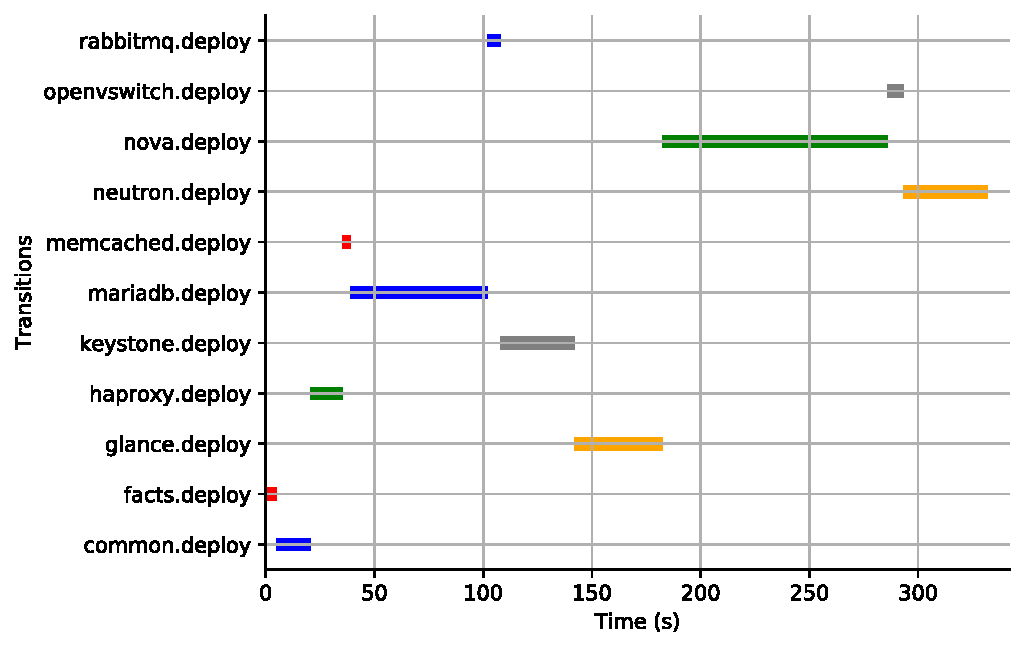
\includegraphics[scale=0.5]{./images/use_case_gantt_cached_ansible.pdf}}
			\label{fig:gantt_ansible}
		}
		%\vspace{-3em}
		\def\svgwidth{\columnwidth}
		\scriptsize
		\subfloat[\aeoass with \emph{cached} registry]{
			\scalebox{0.9}{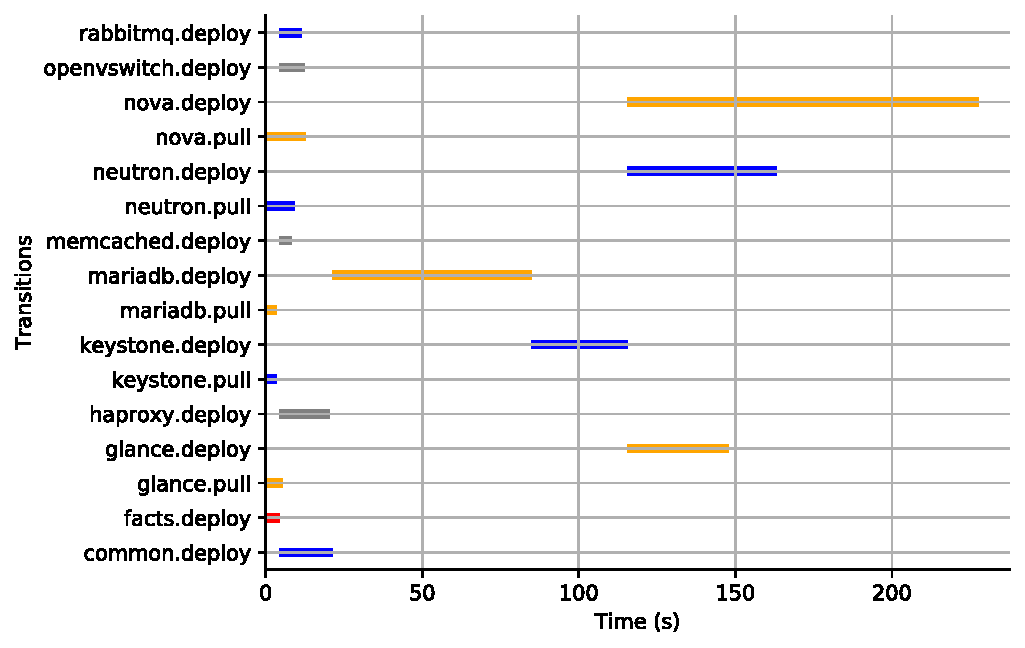
\includegraphics[scale=0.5]{./images/use_case_gantt_cached_aeolus.pdf}}
			\label{fig:gantt_aeolus}
		}
		\caption{(a), (b) Gantt charts of the OpenStack
			commissioning for \ansass, \aeoass with the
			registry set in \emph{cached}.}
		\label{}
	\end{center}
\end{figure*}

To go further, we propose to analyze the
commissioning process at the level of transitions (\ie tasks). To
investigate this aspect, we implemented in \mad the ability to
generate Gantt charts that display the execution time of the different
transitions for each component.
% Maybe something to put in the implementation part
Figures~\ref{fig:gantt_ansible}, \ref{fig:gantt_aeolus},
and~\ref{fig:gantt_madeus} respectively represent the Gantt charts of
the commissioning execution of \ansass, \aeoass and \madass, when the
registry is set to \emph{cached} on \ecotype. Each line of these
figures represents a transition as a function of the elapsed-time
displayed on the X-axis.  First, as previously explained,
Figure~\ref{fig:gantt_ansible} shows that a single transition exists
in each component of the \ansass assembly. Thus, here, each line also
corresponds to one component commissioning. As expected, the figure
shows that each component is deployed in a sequential way. The first
level of parallelism (\ie \emph{SIMH}) is not visible in these figures
since it is handled internally by \ansible playbooks executed in each
transition of the assembly. One can note that Nova, MariaDB, Glance,
Keystone and Neutron take particularly long to commission. 

\aeoass and \madass accelerate the process by (i) splitting the
transition of components into smaller ones and (ii) managing
dependencies between them more finely (depending on the ability to express
\emph{inter-comp}, \emph{inter-comp-tasks} and \emph{intra-comp-tasks}
parallelism).
%
Figure~\ref{fig:gantt_aeolus} illustrates that the components we
highlighted previously (\eg Nova in yellow, Neutron in gray) are based
on two transitions in \aeoass. This figure shows that this assembly
can leverage both the \emph{inter-comp} and \emph{inter-comp-tasks}
parallelism levels since multiple components and
tasks (\eg \texttt{glance.pull} and
\texttt{haproxy.deploy}) are executed in parallel. As a consequence,
the commissioning time drops from $5$ minutes $31$ seconds to $3$
minutes $49$ seconds.

\begin{figure*}[t]
	\begin{center}
		%\vspace{-3em}
		\def\svgwidth{\columnwidth}
		\tiny
		\subfloat[\madass with \emph{cached} registry]{
			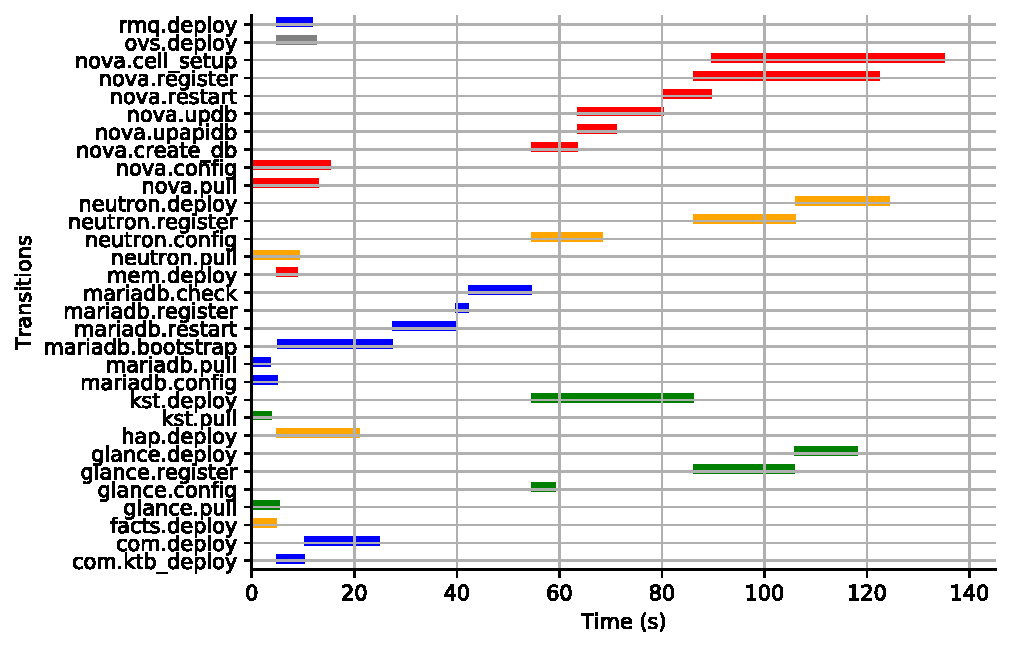
\includegraphics[scale=0.6]{./images/use_case_gantt_cached_mad.pdf}
			\label{fig:gantt_madeus}
		}
		\def\svgwidth{\columnwidth}
		\tiny
		\subfloat[\madass with \emph{remote} registry]{
			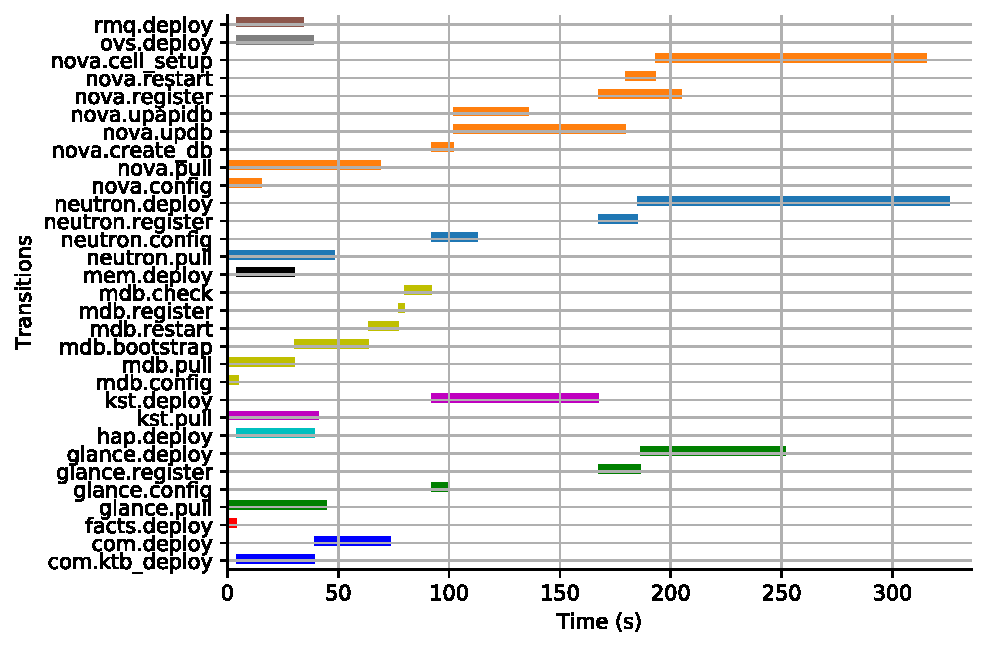
\includegraphics[scale=0.6]{./images/use_case_gantt_remote_madeus.pdf}
			\label{fig:gantt_madeus_remote}
		}
		\caption{(a) Gantt charts of the OpenStack
			commissioning for \madass with the
			registry set in \emph{cached}; (b) Gantt chart of the OpenStack
			commissioning for \madass, with the registry set in
			\emph{remote}.}
		\label{}
	\end{center}
\end{figure*}

Finally, Figure~\ref{fig:gantt_madeus} clearly shows how \mad
leverages the fourth level of parallelism (\ie \emph{intra-comp-tasks}
parallelism) by displaying multiple transitions executed in
parallel. For instance, \texttt{nova.pull} and
\texttt{nova.config} (depicted in orange), are performed
simultaneously which is not possible with \ansible
or \aeolus. Consequently, the commissioning time drops from $5$
minutes $31$ seconds to $2$ minutes $8$ seconds.
%

%-------
\paragraph{Precision of the performance model}
% Construire un tableau contenant les valeurs min/max/moy_obs/moy_calc
The maximum and minimum values obtained by the performance model
described previously is depicted in
\cref{tab:openstack_results_ecotype} and \cref{tab:openstack_results_nova}. These theoretical values are computed
from the average minimum and maximum transitions execution times
observed for the ten experiments of each benchmark. When analyzing
these results, one can note that the measured mean is always
between the expected maximum and minimum.

% donner un exemple ici - peut être développé précedemment dans la partie modèle
% de performance, ou intro pour motiver la contribution du modèle de perf ?

%-------
\paragraph{Influence of registry modes}

\begin{table}
  \begin{center}
    \begin{tabular}{lccc}
      \toprule
      & cached & local & remote\\
      \midrule
      \emph{pull}(s) & 13 & 48 & 52\\
      \emph{pull}(\%) & 10\% & 32\% & 35\%\\
      \bottomrule
    \end{tabular}
    \caption{Time spent in the \emph{pull} transition from Nova and
    percentage compared to the total time for \madass commissioning.}
    \label{tab:pull}
  \end{center}
\end{table}
% TODO: Update these values with last results
% TODO: Give the number for aeolus rather than ansible?
\Cref{tab:openstack_results_ecotype} contains the gains relatively to \ansass,
associated to Figure~\ref{fig:ecotype}. This table shows that the gain
obtained with \emph{local} and \emph{remote} registries are better
than the one obtained with \emph{cached} \docker images.

%\HC[Dimitri]{pourquoi comparer les figures Aeolus ici et non pas
%  Madeus, c'est un peu bizarre je trouve, est-ce que le tableau donne
%  les proportions pour Aeolus ou Madeus ?}
To better understand the origin of this difference, we can compare
Figure~\ref{fig:gantt_madeus} and
Figure~\ref{fig:gantt_madeus_remote}. The former depicts the time
spent by all transitions of \madass, on \ecotype, when the \docker
registry is set on \emph{cached}, while it is set to \emph{remote} for
the latter. As we can see on the figures, the difference is mainly due
to the parallel execution of \texttt{pull} transitions which are much
longer in \emph{remote} (and similarly in \emph{local}) than in
\emph{cached} where images are already on nodes.

\Cref{tab:pull} represents the execution time of
transition \texttt{pull} of the Nova component on \ecotype, as well as
the percentage compared to the total sequential execution time with
\madass. Transition \texttt{nova.pull} takes $35\%$ of the total
commissioning time in \emph{remote}, and only $10\%$ in
\emph{cached}. This confirms that the time spent in
transition \texttt{nova.pull} is much larger for \emph{local} and
\emph{remote} than for \emph{cached}. Thus, the gain
when parallelizing theses transitions is proportionally higher for
\emph{local} and \emph{remote}. This result illustrates the benefit
of parallelizing data transfers in container-based commissionings when
the network bandwidth is sufficient.

Finally, we observe that the global commissioning time for OpenStack
is lower on \ecotype than on \nova. This is due to superior hardware
capabilities for the former, as detailed in \cref{tab:g5k}. Indeed
as \mad introduces more parallelism in the commissioning procedure of
OpenStack, the better the configuration of the cluster, the better the
performance. We argue that the physical nodes on which complex
distributed software systems are deployed often have very powerful
hardware, and that exposing more parallelism in the
commissioning process is an additional way to exploit their high
performance level.

%\HC[Helene]{J'enlèverai la partie qui suit car ce n'est pas très
%  précis, on a testé sur 2 clusters pour valider les résultats tout simplement.}

%  ------
\paragraph{OpenStack Continuous Integration}

To highlight the potential gain in real-world situations, we apply the
above results to the traces of the OpenStack CI. Traces of the
OpenStack Continuous Integration
platform\footnote{\url{http://logstash.openstack.org}} have been
recorded through an automated \python script over nine days from
Februrary 19 to February 27, 2020 with specific requests regarding
the \kolla project. The script, as well as well as the raw data
obtained from the requests, are available in the reproducible lab of
the paper. Figure~\ref{fig:oci} shows the accumulated number of \kolla
deployments for each day. Exactly 2963 deployments have been recorded
in nine days, an average of 329 runs per day.


\begin{figure}[tbp]
	\begin{center}
		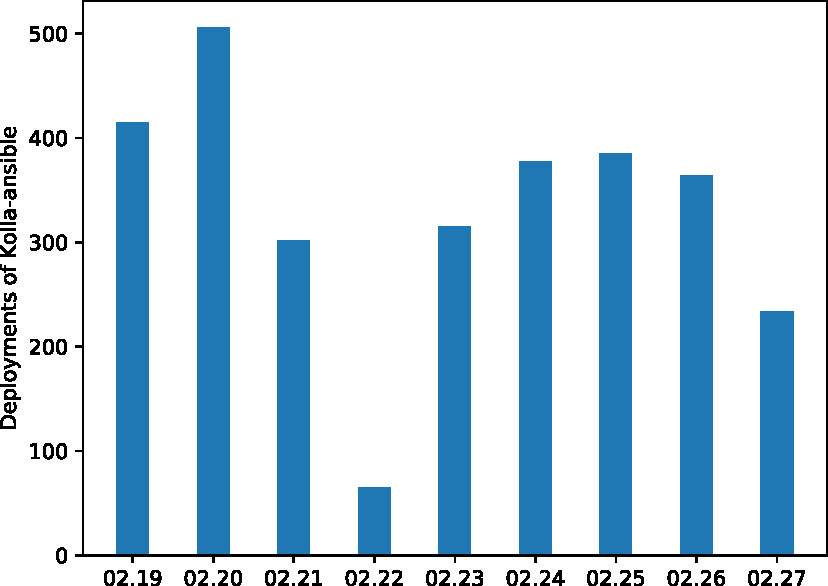
\includegraphics[width=0.9\linewidth]{./images/kolla_deployments.pdf}
	\end{center}
	\caption{Traces recorded from the OpenStack CI platform over nine days on the 
	deployment of the \kolla project.}
	\label{fig:oci}
\end{figure}

The Openstack CI log servers process a large amount of data coming from all
the Openstack projects and only store up to 7 days of logs. The script makes
requests for all the logs coming from the kolla-ansible project and aggregates
them by build uuid, a unique identifier for each build on the Openstack CI,
allowing us to count the number of CI operations related to the project.
Because some CI operations do not generate a full Openstack deployment, we filter
these results to gather the CI events from the kolla-ansible project that are
longer than 15 minutes, which is a good indicator that an Openstack deployment
happened.

Table~\ref{tab:projection} illustrates the projection of the gain based on these 
traces, when considering the deployment times of our experiments in \emph{remote} mode. 
Of course the OpenStack CI traces probably also include additional tests, and 
deploy more complex versions of OpenStack, but we only illustrate the 
possible gain according to our results. 

\begin{table}
\begin{center}
	\begin{tabular}{lccc}
		\toprule
		& \kolla & \mad & gain\\
		\midrule
		\emph{reference time}(s) & 529 & 150 & 71\%\\
		\emph{projection on 9 days}(h) & 435 & 123 & 71\%\\
		\emph{projection on av./day}(h) & 48 & 14 & 71\%\\
		\bottomrule
	\end{tabular}
	\caption{Projection of the OpenStack CI traces with our reference experimental 
			measurements with \emph{remote} mode on \ecotype 		
			(Table~\ref{tab:openstack_results_ecotype}). Traces of 			
			Figure~\ref{fig:oci} on the deployment of \kolla over nine days in 
			Frebruary 2020 are used with a total of 2963 \kolla run in 9 days and 
			an average of 329 runs per day.}
			\label{tab:projection}
	\end{center}
\end{table}

Over nine days a total of 312 hours of computations could have been
saved on the CI platform, 34 hours per day on average.  Finally, one
should note that the recorded period was not particularly active as no
OpenStack release was close. It is likely that a higher number
of \kolla runs will be recorded on the CI platform in periods leading
up to a release.
%This could be verified for the next release 9.0.2 of OpenStack.

%-------
% \paragraph{Impact of underlying clusters}

% To better understand the impact of the underlying clusters, we can study
% \cref{fig:openstack_results} which compares the results obtained on \ecotype and
% \nova. First, the global time for OpenStack commissioning is lower on \ecotype
% than on \nova. This is due to a better hardware configuration for the former,
% regarding CPU, RAM and network, as detailed in \cref{tab:g5k}.

% Furthermore, the gain is higher for results obtained on \ecotype than on \nova.
% Since our contribution enables a high degree of parallelism during the
% commissioning process, the ability for cluster nodes to manage parallelism has
% an impact on the performance.
% It is well known that introducing too much parallelism can have a negative
% impact on the performance because of the overhead of parallelism management.
% The results on \nova are thus less convincing than the results obtained on
% \ecotype.  By monitoring CPU, memory, and bandwidth usage on an outdated
% hardware configuration, we could have observed that some nodes have their memory
% and/or CPU saturated.
% Hence, the actual benefits of \mad depends on the possibility to efficiently
% exploit the available parallelism.

